\subsection{Timeline}
Questa timeline contiene i passi più importanti della diffusione del worm, e bisogna notare la presenza di due diverse versioni di Code Red che sono state rilasciate in quel periodo:
\begin{itemize}
\item[-]18 giugno: eEye Security rende nota pubblicamente la vulnerabilità dei web server IIS;
\item[-]26 giugno: Microsoft rilascia una patch per risolvere la vulnerabilità;
\item[-]12 luglio: una prima versione del worm “Code Red” viene rilasciata, residente in memoria, seme statico, scanning randomico;
\item[-]19 luglio: il worm “CodeRed v2” viene rilasciato con seme dinamico.
\end{itemize}
%%%%%%%%%%%%%%%%%%%%%%%%%%%%%%%%%%%%%%%%%%%%%%%%%%%%%%%%%%%%%%%%%%%%%%%%%%%%%%%%%%%%%%%%%%%%%%%
\subsection{Caratteristiche e comportamento}
Il payload dei pacchetti provenienti dal worm si presenta nel seguente modo (figura~\ref{payload}):
\begin{figure}[!h]
\centering
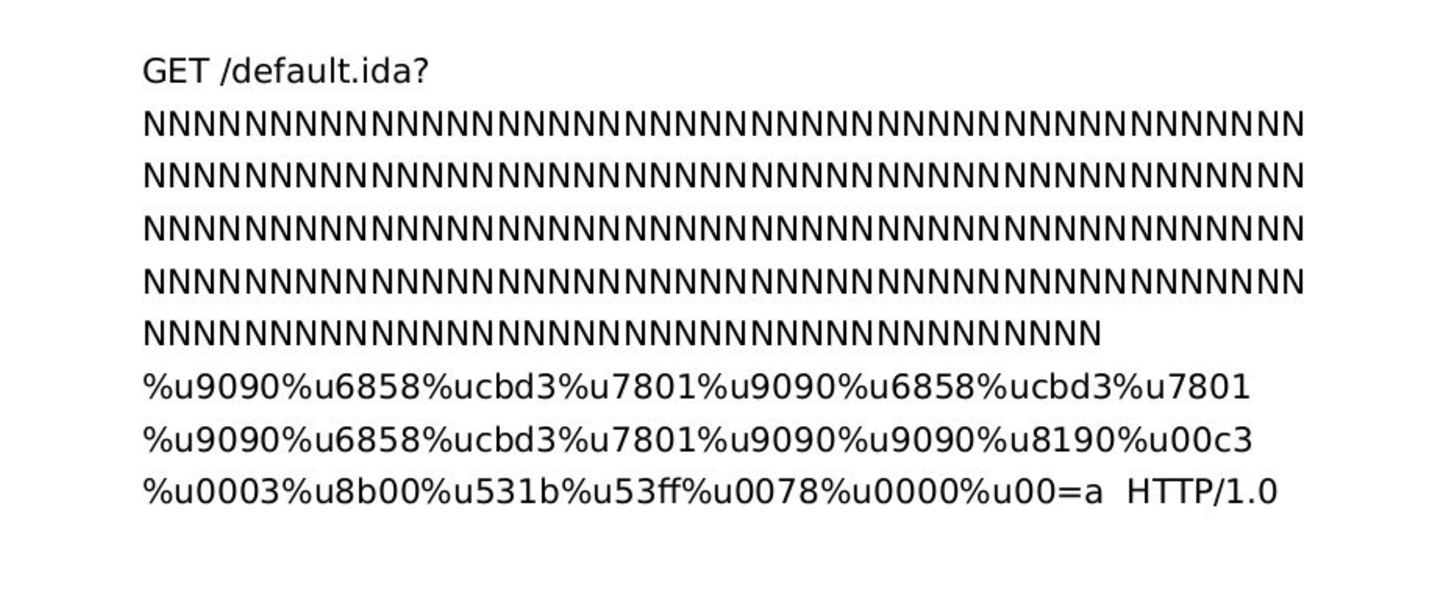
\includegraphics[width=0.8\textwidth]{images/payload.eps}
\caption{payload}
\label{payload}
\end{figure}
La serie di “N” con cui inizia il payload serve esclusivamente per generare l’overflow del buffer, mentre l’istruzione vera e propria, inserita dall’attaccante, è la parte seguente. A causa dell’overflow l’host interpreta le stringhe come istruzioni, le esegue portando all’esecuzione del comando arbitrario inserito dall’attaccante.

La caratteristica del worm Code Red è il suo comportamento dinamico, dipendente dal giorno del mese. Lo schema utilizzato è il seguente:
\begin{itemize}
\item[-]Giorni 1-19 : il worm prova a diffondersi cercando altri server IIS nella rete Internet;
\item[-]Giorni 20-27 : sfrutta le macchine che è riuscito ad infettare per lanciare un attacco DDoS contro diversi indirizzi IP (incluso quello della Casa Bianca 198.137.240.91);
\item[-]Giorni 28-fine del mese: va in “sleep”.
\end{itemize}
%%%%%%%%%%%%%%%%%%%%%%%%%%%%%%%%%%%%%%%%%%%%%%%%%%%%%%%%%%%%%%%%%%%%%%%%%%%%%%%%%%%%%%%%%%%%%%%
\subsection{Diffusione}
La diffusione è un aspetto critico per il worm Code Red. Lo schema seguito è il seguente:\\
\begin{enumerate}
\item Setup dell’ambiente iniziale del worm nel sistema infetto
\item Vengono creati 100 thread:
\begin{itemize}
\item[-]i primi 99 vengono usati per diffondere il worm attraverso la creazione di indirizzi IP randomici.
\item[-]il 100-esimo controlla la versione del sistema operativo (Windows NT/2000) del sistema in cui è in esecuzione:
i. se il sistema operativo è di lingua Inglese(US), la pagina web del web server viene cambiata figura~\ref{hacked}, e tale modifica resta attiva per 10 ore prima di sparire
ii. in caso contrario il 100-esimo thread si unisce agli altri 99 per diffondere il worm
\end{itemize}
\item Ogni thread controlla la presenza del file c:$\backslash$notworm
\begin{itemize}
\item[-]se il file è trovato, il worm va in sleep
\item[-]altrimenti i thread continuano nel processo di infezione di altri sistemi
\end{itemize}
\item Ogni thread controlla l’ora del sistema 
\end{enumerate}
Entrambe le versioni rilasciate del worm hanno utilizzato lo stesso schema, con la sola differenza del seme usato per generare indirizzi casuali, che è statico nella prima versione e dinamico nella seconda. Questo dettaglio è di fondamentale importanza, ed è stato il cambiamento vincente della seconda versione per ottenere una rapida diffusione su scala mondiale.\\
\begin{figure}[!h]
\centering
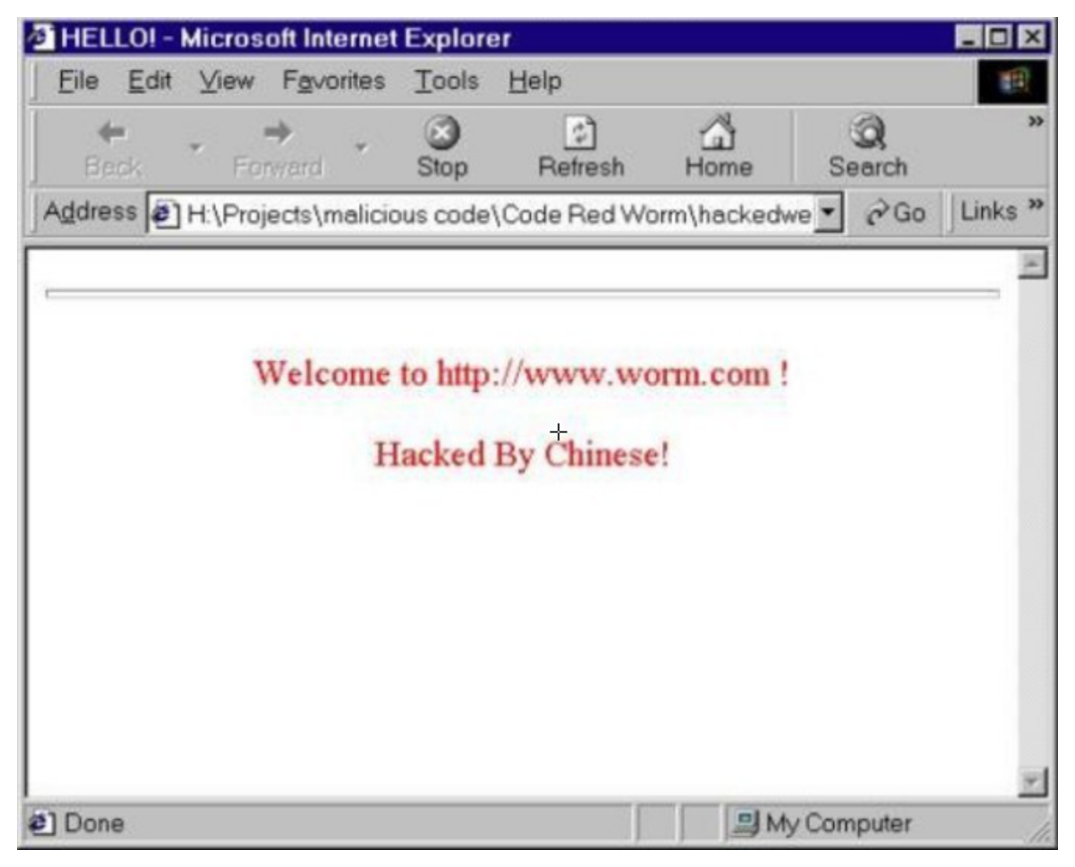
\includegraphics[width=0.7\textwidth]{images/hacked.eps}
\caption{defacing della pagina web}
\label{hacked}
\end{figure}
\subsection{Vulnerabilità}
La vulnerabilità è rappresentata da un buffer senza controllo sulla dimensione relativa alle richieste in arrivo, ed è presente in alcune estensioni ISAPI\footnote{L’ISAPI (Internet Services Application Programming Interface) è una tecnologia che permette agli sviluppatori di estendere le funzionalità fornite dal server IIS.} associate a “Microsoft Index Server” e “Indexing Service”\footnote{Microsoft Index Server e Indexing Service sono motori di ricerca e di indicizzazione. Permettono agli utenti di ricercare dati nei siti web o nei server web inserendo parole chiave, frasi o proprietà nei web browser.}. Il primo appartiene a “Windows NT 4.0 Option Pack” mentre il secondo è un servizio nativo di “Windows 2000”.\\
Un host che esegue una delle due può subire l’esecuzione di codice arbitrario a causa di tale vulnerabilità nell’estensione ISAPI idq.dll\footnote{Un estensione ISAPI è una dynamic link library (.dll) che usa ISAPI per fornire un set di funzioni web al di sopra di quelle fornite nativamente da IIS.\\
Idq.dll fornisce supporto per i file .ida-Internet Data Administration and .idq Internet Data Query.}. Questi processi sono eseguiti nel Local System context, permettendo all’attaccante di eseguire codice con privilegi Local System. Lo sfruttamento di questa vulnerabilità porta l’host target ad essere completamente compromesso in quanto l’attaccante potenzialmente può: eseguire codice arbitrario nel server, cambiare i contenuti contenuti in esso e riconfigurarlo.\\
Non serve che Index Server e Indexing Service siano in esecuzione per sfruttare la vulnerabilità, perché idq.dll è installato di default quando viene installato Microsoft IIS-Internet Information Server, quindi basta l’esecuzione di quest’ultimo.\\
%%%%%%%%%%%%%%%%%%%%%%%%%%%%%%%%
\subsubsection{Dettagli tecnici}
Nel suo processo di installazione, l’IIS installa diverse estensioni ISAPI, tra cui le “.dll” che forniscono funzionalità aggiuntive.
Quando un utente deve usare una funzione dell’estensione ISAPI manda una richiesta al server, anche se a volte è possibile chiamare l’estensione ISAPI direttamente. La richiesta dell’utente viene analizzata e IIS determina l’estensione ISAPI da usare, consultando una tabella con i mapping tra le estensioni dei file e ogni estensione ISAPI sul server.\\
L’estensione ISAPI che contiene la vulnerabilità è idq.dll, la quale fornisce due funzioni:
\begin{itemize}
\item[-]fornisce supporto per i file .ida (Internet Data Administration), che sono script che possono essere usati per gestire l’Indexing Service;
\item[-]processa i file .idq (Internet Data Query), usata per implementare ricerche custom.
\end{itemize}

Per sfruttare la vulnerabilità deve esistere un mapping tra i file .idq e .ida con l’ idq.dll.\\
Un attaccante che può stabilire una connessione con un server su cui è installato l’idq.dll, può condurre un attacco sfruttando tale vulnerabilità, riuscendo ad eseguire codice arbitrario sul server.\\
C’è un buffer non controllato nella parte di codice che gestisce le richieste in arrivo. L’arrivo di una richiesta “malformata” causerà un risultato diverso in base al tipo di contenuto della richiesta stessa:
\begin{itemize}
\item[-]dati randomici causeranno il fallimento del server. Nel caso di IIS 4.0 servirà l’intervento dell’amministratore, altrimenti nel caso di IIS 5.0 il server web sarà in grado di ripristinarsi in modo autonomo;
\item[-]codice eseguibile arbitrario causerà la sua esecuzione nel server web.
\end{itemize}

L’attaccante ottiene pieno controllo del server web, può eseguire ogni azione che desidera perché l’idq.dll è eseguito nel System Context.\\

A causa dei seri rischi legati a tale vulnerabilità, Microsoft ha consigliato agli utenti potenzialmente interessati da essa di prendere tempestive azioni di protezione. E’ stata rilasciata una patch per eliminare la vulnerabilità, mentre per i clienti impossibilitati ad installarla si poteva ricorrere alla rimozione dei mapping con i file .idq e .ida attraverso l’Internet Services Manager in IIS. Quest’ultima soluzione tuttavia non è da considerarsi come definitiva, in quanto a seguito di aggiunta/rimozioni di componenti addizionali di sistema poteva avvenire il reinserimento automatico dei mapping dannosi.\\

Chi può sfruttare la vulnerabilità? Attraverso essa può avere controllo sulla rete intera?\\
L’attaccante deve essere solo in grado di imporre una richiesta all’idq.dll . La presenza del mapping che associa i file .idq e .ida ad idq.dll, permette all’attaccante di stabilire una sessione web con il server, attraverso cui sfruttare la vulnerabilità.
Ci sono delle “best-practice” che aiutano a limitare la portata dell’intromissione di un attaccante. I web server, soprattutto quelli pubblici, sono sempre stati tra i target preferiti degli attacchi a causa della loro esposizione nella rete. Bisogna tenerne conto nel design della rete, e il primo obiettivo dev'essere quello di limitare le possibili conseguenze della compromissione di un server web.\\
In particolare si seguono due pratiche:
\begin{itemize}
\item[-]Isolare i web server nelle DMZ\footnote{una DMZ (DeMilitarized Zone) è una sottorete isolata, fisica o logica, la quale contiene dei server con lo scopo di renderli accessibili senza compromettere la sicurezza della rete.}, separandoli quindi dal resto della rete;\\
\item[-]Configurarli come macchine “stand-alone”. Se necessariamente devono far parte di un dominio, questo deve contenere solo macchine della DMZ. I web server non dovrebbero mai far parte dei più grandi domini nella rete.\\
\end{itemize}
Queste pratiche negano all’attaccante di arrivare facilmente al server, ma in caso di attacco riuscito questo potrebbe usare il server “conquistato” per attaccare altre macchine.\\
%%%%%%%%%%%%%%%%%%%%%%%%%%%%%%%%
\subsubsection{Fattori mitiganti}
\begin{itemize}
\item[-]La vulnerabilità può essere sfruttata solo se viene stabilita una sessione web con un server infetto. Per essere a rischio bisogna avere IIS, e questo è il caso di Windows 2000 Professional;
\item[-]La vulnerabilità non può essere sfruttata se non sono presenti i mapping con i .ida e .idq . Tali mapping possono essere rimossi come detto in precedenza;
\item[-]L’abilità di un attaccante che ha compromesso un web server è legata fortemente dall’architettura di rete. La “best practice” per l’architettura di rete riguardo le macchine da proteggere come i web server, prevede di minimizzarne l’esposizione verso un ambiente non controllato come Internet, posizionandole in DMZ, isolandole il più possibile dal resto della rete. Questa pratica può limitare pesantemente il raggio di azione di un attaccante.
\end{itemize}
